\usepackage[authoryear,round]{natbib}
\usepackage{multirow}

\newcommand{\sheetnum}{%
	12
}
%\setcounter{section}{\sheetnum-3}
\newcommand{\tutorialtitle}{%
    Inference  \&
    Bayesian networks
}
\newcommand{\tutorialtitleshort}{%
	Intro Bayesian nets
}
% for slides
\subtitle{\sheetnum \tutorialtitle}

%\maxdeadcycles=1000 % Workaround for ! Output loop---100 consecutive dead cycles because of too many figures

% The following use of algroithms does not work well with the notes:
%
%
%
%
% instead use the following for your algorithms:
%
%\begin{figure}[!t]
%\removelatexerror
%\begin{algorithm}[H]
    % your algo here
    %\label{alg:algolabel}
    %\caption{algocaption}
%\end{algorithm}
%\end{figure}
%\begin{algorithm}
% Below is the definition for the command \removelatexerror:
\makeatletter
\newcommand{\removelatexerror}{\let\@latex@error\@gobble}
\makeatother

\begin{document} %%%%%%%%%%%%%%%%%%%%%%%%%%%%%%%%%%%%%%%%%%%%%%%%%%%%%%%

\sheet{\sheetnum}{\tutorialtitleshort}

\ttopic{\tutorialtitle}

\columnratio{0.2,0.8}\textbf{}
\begin{paracol}{2}
%\setlength{\columnseprule}{0.1pt}
%\setlength{\columnsep}{5em}

\begin{rightcolumn}

% notes version will ignore it
\begin{frame}
\titlepage
\end{frame}

\begin{frame}
\tableofcontents
\end{frame}

\mode<all>
\section{Inference and Uncertainty}

\mode<presentation>{
\begin{frame} 
    \begin{center} \huge
        \secname
    \end{center}
    \begin{center}
    quanitfying degree of belief/\\
    quanitfying uncertainty
    \end{center}
\end{frame}
}

\subsection{The probabilistic model}

\begin{frame}\frametitle{\subsecname}

\begin{itemize}
    \item \underline{The model:}\\
        \begin{align}
            P(H): H \rightarrow [0,1]&&\\
            P(H) = 0 && \iff H \text{ is false (i.e. impossible)} \\
            P(H) = 1 && \iff H \text{ is true (i.e. certain)} \\
            0 < P(H) < 1 && \text{quantifies our degree of belief}
        \end{align}
    \pause
    \item \textbf{events}: assignment to a set of cases\\
    (e.g. two dice add up to 11)
    \pause
    \item \textbf{proposition}: disjunction of \textbf{events}\\
    (i.e. isolate the sets of \textbf{events} in which the \textbf{proposition} holds)\\
    
\end{itemize}
    
\end{frame}

\begin{frame}

$\underbrace{\text{\emph{Summing over}}}_{\text{marginalisation}}$ the probabilities of the \textbf{events} $\leadsto$ probability of \textbf{proposition}.\\

Example:

\begin{align}
P(\text{Total} = 11) &= P(\text{Die}_{1} = 5, \text{Die}_{2} = 6) + P(\text{Die}_{1} = 6, \text{Die}_{2} = 5)\\
        &\stackrel{\text{shorthand}}{=} P(5,6) + P(6,5)\\
        &= 1 / 36 + 1/36\\
        &= 1/18
\end{align}

$P(\text{Total} = 11), P(5,6) \text{ and } P(6,5)$ are \emph{unconditional} or \emph{prior} probabilities.\\
They represent the degree of belief in the absence of any other information.\\
Priors is also referred to as \emph{domain knowledge}.
        
\end{frame}

\subsection{Evidence}

\begin{frame}\frametitle{\subsecname}

What if we already \emph{know} (i.e. observed) something?\\

e.g. We've already rolled the first die and got 5.\\
Now we're waiting to roll the second die.\\

We are now interested in the \emph{conditional} (or \emph{posterior}) probability of the second die leading to a total of 11:

\begin{equation}
P(\text{Total}= 11) \underbrace{\big|}_{\text{``given''}} \overbrace{\text{Die}_{1}}^{\mathclap{\{1,2,3,4,5,6\}}} = 5)
\end{equation}

\end{frame}

\begin{frame}\frametitle{A thing about priors}

The prior is valid event after the outcome.

e.g.\\
\begin{itemize}
 \item[] $P(\overbrace{cavity}^{\text{Cavity}=1}) = 0.2$
 \item[] $P(cavity | \overbrace{toothache}^{\text{Toothache}=1}) = 0.6$
 \item[] If we observe that a cavity has actually occured, we don't have to change our prior on cavities.\\
 However, the prior becomes less useful if we proceed to infer other things.
\end{itemize}
    
\textbf{Caution}\\
\begin{itemize}
\item[$\times$] Whenever Toothache is true, then cavity is true with probability of 0.6
\item[\checkmark] Whenever Toothache is true, \textit{and no other information} is available, then cavity is true with probability of 0.6.
\end{itemize}

\textit{other information}: Diagnosis was \underline{no} cavity. In this case, the probability is no longer 0.6, but:
\begin{equation}
P(cavity | toothache \wedge Diagnosis cavity = false) = 0
\end{equation}

\end{frame}

Observing event $e$ rules out events where e is false. This leaves a set where $P(e)>0$.
We look within that set for the fraction that satisfies $x$ and $e$.

This fraction can be calculated using the following:

\begin{equation}
P(x|e) = \frac{P(x,e)}{P(e)}
\end{equation}

which brings us to the \emph{product rule}:

\begin{equation}
P(x,e) = P(x|e) P(e)
\label{eq:productrule}    
\end{equation}


\begin{frame}

\question{What information do I need to calculate the probability of any proposition?}

- The full joint probability distribution\notesonly{ provides all the information to calculate the probability of any proposition.}

Example:\\

%\footnotesize
	%\begin{center}
     \begin{table}[h] 
	\begin{tabular}{|c|c|c|}
		\hline
		& $toothache = \text{true}$ & $toothache = \text{false}$ \\
		\begin{tabular}{c}
			\\ 
			$cavity = \text{true}$ \\
			$cavity = \text{false}$
		\end{tabular} 
		& 
		\begin{tabular}{c|c}
			$catch = \text{true}$ & $catch = \text{false}$\\ 
			\hline 
			$0.108$ & $0.012$ \\
			$0.016$ & $0.064$
		\end{tabular} 
		& 
		\begin{tabular}{c|c}
			$catch = \text{true}$ & $catch = \text{false}$\\ 
			\hline 
			$0.072$ & $0.008$ \\
			$0.144$ & $0.576$
		\end{tabular} 
		\\ \hline
	\end{tabular}
    \end{table}
	

\end{frame}

\subsubsection{Marginalisation}



\begin{frame}\frametitle{\subsubsecname~(``summing out'')}

\notesonly{\subsecname~$\corresponds$~``summing out''}

\begin{align}
P(x | \vec e)
&= \frac{x, \vec e}{P(\vec e)}\\
&= \alpha \sum_{\vec y \in \vec Y} P(\vec x, \vec e, \vec y)
\end{align}

where
\begin{itemize}
\item[] $x$: query variable
\item[] $\vec e$: evidence variable(s)
\item[] $\vec y$: \textbf{un}observed variables in the table
\item[] $\alpha$: normalization factor:

\question{How do we calculate the normalization factor $\alpha$?}

- Via
\begin{enumerate}
\item evidence prior:
\begin{equation}
\alpha := P(\vec e) = \sum_{x, \vec y} P(x, \vec e, \vec y)  
\end{equation}
\item or simply via whatever ensures $\sum_{\vec x} P(x, \vec e) = 1$
\end{enumerate}

\end{itemize}
    
\end{frame}

\subsubsection{Applying the product rule}

\begin{frame}\frametitle{\subsubsecname}
    
\begin{align}
P(cavity | toothache=true) &= \frac{cavity,toothache}{P(toothache)}\\
&= \frac{0.108 + 0.012}{0.108 + 0.012 + 0.016 + 0.064}\\
&= 0.6   
\end{align}


\begin{equation*}
P(cavity=false | toothache=true) = ?
\end{equation*}

\question{What should we expect?}

\pause

\begin{align}
P(cavity=false | toothache=true) &= \frac{cavity=false,toothache}{P(toothache)}\\
&= \frac{0.016 + 0.0064}{0.108 + 0.012 + 0.016 + 0.064}\\
&= 0.4 = 1 - 0.6   
\end{align}

\textbf{Remark}: The denominator remains constant no matter which value of cavity we are interested in.\\
$\Rightarrow$ use $1/P(toothache)$ as the normalization factor for $P(cavity | toothache)$.

\begin{align}
P(Cavity|toothache) &= \alpha P(Cavity, toothache) \\
&= \alpha \big\lbrack
P(Cavity, toothache, catch) + P(Cavity, toothache, catch=false) 
\big\rbrack\\
&= \alpha \big\lbrack{}
\rmat{0.108\\0.016} + \rmat{0.012\\0.064}
\big\rbrack\\
&= \alpha \rmat{0.12\\0.08} \stackrel{\alpha=1/P(toothache)}{=} \rmat{0.6\\0.4}
\intertext{OR normalize s.t. $\sum_{\vec x} P(x, \vec e) \eqexcl 1$}
&= \alpha \rmat{0.12\\0.08} \stackrel{\alpha=\frac{1}{0.12+0.08}}{=} \rmat{0.6\\0.4}
\end{align}



\end{frame}

\mode*

\mode<all>
\section{Independence}

\definecolor{darkgreen}{rgb}{0,0.6,0}

\mode<presentation>{
\begin{frame} 
    \begin{center} \huge
        \secname
    \end{center}
    $$P(X,Y) = P(X)P(Y)$$
\end{frame}
}

\subsection{Motivation}

\begin{frame}\frametitle{\secname:~\subsecname}

The full joint distribution has everything we need to perform inference,
but it scales badly with more and more variables (e.g. adding $\mathit{Weather}$ (e.g. \# of weather conditions = 4) leads to a table with $2\times2\times2\times4=32$ entries)

\pause

\question{Should the weather be influenced by a $\mathit{cavity}$?}

\pause

\slidesonly{\vspace{-5mm}}

\begin{equation}
P(\mathit{cloudy} | \mathit{toothache}, \mathit{catch}, \mathit{cavity}) \stackrel{!}{=} P(\mathit{cloudy})
\end{equation}

\pause

\question{Should the weather have any influence on cavities, $\mathit{toothache}$ or the dentist?}

\pause

\notesonly{
-No, this independence can be formulated by:
}

\slidesonly{\vspace{-5mm}}

\begin{align}
P(\mathit{toothache}, \mathit{catch}, \mathit{cavity}, \mathit{Weather}) &\\
\stackrel{!}{=} P(\mathit{toothache}, &\mathit{catch}, \mathit{cavity})P(\mathit{Weather})
\end{align}


The 32 elements in the table can be split into \notesonly{the original} 8 + 4 \notesonly{(new table with 4 entries for the weather)}.

\end{frame} 

\begin{frame}\frametitle{\secname:~\subsecname}

``Extreme'' case:\\
 $n$ independent coin flips: $2^n$ combinations.\\
 Independence allows us to reduce this to $n \times$ single-variable distributions.

\end{frame}

\subsection{Bayes' theorem}

\mode<presentation>{
\begin{frame} 
    \begin{center} \huge
        \subsecname
    \end{center}
    
    \begin{equation*}
P(Y|X) = \frac{P(X|Y)P(Y)}{P(X)}
\end{equation*}
    
    \begin{center}   
   How do we get there? - product rule\\
     Why is it important? $\Rightarrow$ Conditional independence
    \end{center}
\end{frame}
}

\begin{frame}\frametitle{\subsecname}

Start with the product rule:

\begin{align}
P(X|Y)P(Y) = P(Y,X) &= P(X,Y) \visible<2->{= P(Y|X)P(X)\\
P(X|Y)P(Y) &= P(Y|X)P(X)}
\visible<3->{
\intertext{solve for $P(Y|X)$}
P(Y|X) = \frac{P(X|Y)P(Y)}{P(X)}
}
%\tag{Bayes' theorem}
\label{eq:bayes}
\end{align}

\end{frame}

\begin{frame}\frametitle{How to read Bayes' theorem}
\notesonly{
How to read Bayes' theorem:
}

\mode<presentation>{
    \begin{equation*}
P(Y|X) = \frac{P(X|Y)P(Y)}{P(X)}
\end{equation*}
}

\pause 

\only<2>{


\begin{figure}[h]
     \centering
	 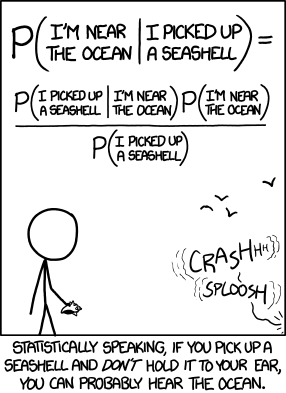
\includegraphics[width=0.33\textwidth]{img/xkcd_seashell}%
	 \caption{Bayes' Theorem example from \href{https://imgs.xkcd.com/comics/seashell.png}{xkcd.com}}
\end{figure}

}

\pause

\begin{equation}
\underbrace{P(\mathit{cause}|\mathit{effect})}_{\text{diagnositc}} = \frac{\overbrace{P(\mathit{effect}|\mathit{cause})}^{\text{causal}}P(\mathit{cause})}{P(\mathit{effect})}
\end{equation}

If $P(\mathit{effect})$ is missing, we can still normalize using:

\begin{equation}
P(Y|X) = \alpha P(X|Y)P(Y)
\end{equation}

$\alpha$ is chosen to whatever will make the entries in $P(Y|X)$ sum up to $1$.


\end{frame}

\subsection{Using Bayes' theorem}

\begin{frame}\frametitle{\subsecname}

\only<1>{
\begin{equation}
P(Y|X) = \alpha P(X|Y)P(Y)
\end{equation}

\begin{align}
P(\mathit{Cavity}|\mathit{toothache}=\text{true}, \mathit{catch}=\text{true}) &\\ 
=\alpha \underbrace{P(\mathit{toothache}=\text{true}, \mathit{catch}=\text{true}}_{\circledast} &| \mathit{Cavity})P(\mathit{Cavity})
\label{eq:applybayes}
\end{align}

$\circledast$ similar scaling problem, not much better then the case of using the full joint distribution.

}

\only<1,2>{

\question{Can we use independence to further mitigate the scaling problem here?}

}

\only<2>{

\begin{center}
$\mathit{Toothache}$ and $\mathit{Catch}$ are not independent.\\
But\\
$\mathit{Toothache}$ given $\mathit{cavity}$ is independent of $\mathit{Catch}$ given $\mathit{cavity}$
\end{center}

\begin{itemize}
\item $\mathit{toothache}$ depends on $\mathit{cavity}$: nerves \& tolerance for pain.
\item $\mathit{catch}$ depends on $\mathit{cavity}$: dependent on how skillful the dentist is.
\item \textbf{But}\ldots
\notesonly{``nerves \& tolerance for pain'' is \underline{independent} of ``how skillful the dentist is''.}
\end{itemize}

%TODO figure

}




\end{frame}

\begin{frame}

\mode<presentation>{
\slidesonly{\vspace{-5mm}
}

\begin{align}
P(\mathit{Cavity}|\mathit{toothache}=\text{true}, \mathit{catch}=\text{true}) &\\ 
=\alpha \underbrace{P(\mathit{toothache}=\text{true}, \mathit{catch}=\text{true}}_{\circledast} &| \mathit{Cavity}) P(\mathit{Cavity})
\label{eq:applybayes}
\end{align}

\begin{itemize}
\item $\mathit{toothache}$ depends on $\mathit{cavity}$: nerves \& tolerance for pain.
\item $\mathit{catch}$ depends on $\mathit{cavity}$: dependent on how skillful the dentist is.
\item \textbf{But}\ldots ``nerves \& tolerance for pain'' is \underline{independent} of ``how skillful the dentist is''.
\end{itemize}
}

Therefore:
\slidesonly{\vspace{-5mm}
}

\begin{align}
P(\mathit{toothache}
%=\text{true}
, \mathit{catch}
%=\text{true}
 | \mathit{Cavity}) &\\
= P(\mathit{toothache}
%=\text{true}
| \mathit{Cavity}) &P(\mathit{catch}
%=\text{true}
| \mathit{Cavity})
\label{eq:condindep}
\end{align}

i.e. \emph{conditional} independence of $\mathit{toothache}$ and $\mathit{catch}$ \underline{given} $\mathit{cavity}$

\pause

Plugging \eqref{eq:condindep} into \eqref{eq:applybayes} yields:

\slidesonly{\vspace{-4mm}}

\begin{align}
P(\mathit{toothache}, \mathit{catch} | \mathit{Cavity}) &\\
= \alpha P(\mathit{toothache}| \mathit{Cavity}) &
P(\mathit{catch}| \mathit{Cavity}) P(\mathit{Cavity})
\end{align}

i.e. \emph{conditional} independence of $\mathit{toothache}$ and $\mathit{catch}$ \underline{given} $\mathit{Cavity}$
\end{frame}

\subsection{Naive Bayes}

\begin{frame}\frametitle{\subsecname}

An alternate expression for the full joint distribution by exploiting conditional independence.

We start with the product rule:

\begin{equation}
P(X,Y) = P(X|Y)P(Y)    
\end{equation}

\begin{equation}
P(\mathit{Toothache},\mathit{Catch},\mathit{Cavity}) = P(\mathit{Toothache},\mathit{Catch}|\mathit{Cavity}) \underbrace{P(\mathit{Cavity})}_{\text{prior}} 
\end{equation}

Exploiting conditional independence yields:

\begin{align}
P(\mathit{Toothache},\mathit{Catch},\mathit{Cavity}) &\\
= P(\mathit{Toothache}|\mathit{Cavity}) &P(\mathit{Catch}|\mathit{Cavity}) \underbrace{P(\mathit{Cavity})}_{\text{prior}} 
\end{align}

\end{frame}

\begin{frame}\frametitle{\subsecname}

\mode<presentation>{
\begin{align*}
P(\mathit{Toothache},\mathit{Catch},\mathit{Cavity}) &\\
= P(\mathit{Toothache}|\mathit{Cavity}) &P(\mathit{Catch}|\mathit{Cavity}) \underbrace{P(\mathit{Cavity})}_{\text{prior}} 
\end{align*}
}

In terms of cause and effect:

\begin{align}
P(\mathit{Cause}, \mathit{Effect}_1, \mathit{Effect}_2,\ldots, \mathit{Effect}_n) &\\
= \underbrace{P(\mathit{Cause})}_{\text{prior}} &\prod_{i=1}^{n} P(\mathit{Effect}_{i}|\mathit{Cause})
\end{align}

Complexity reduced!

\end{frame}

\mode*

\clearpage

\mode<all>
\section{Bayesian Networks (part 1/2)}



\mode<presentation>{
\begin{frame} 
    \begin{center} \huge
        \secname
    \end{center}
    \begin{center}   
    Towards an efficient representation of the full joint distribution that exploits conditional independence
    \end{center}
\end{frame}
}



% =============================================================================
\subsection{Directed Acyclic Graphs (DAG)}


\begin{frame}\frametitle{\subsecname}

A graphical representation of conditional independence:
\begin{figure}[h]
	\centering
	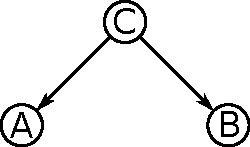
\includegraphics[width=0.3\linewidth]{img/cond}%
	\notesonly{
	\caption{
	The conditional independence between $A$ and $B$ given $C$.
	}%
	}%
    \label{fig:cond}%
\end{figure}

This leads to the factorization of the full joint distribution:

\begin{equation}
P(A,B,C) = P(A|C)P(B|C)P(C)
\end{equation}

\end{frame}


\begin{frame}\frametitle{\subsecname}
    
\question{What does the DAG representation of this full joint distribution look like for toothache example?}

(\textbf{see blackboard})

\end{frame}

\subsubsection{A ``Californian'' example}

% -----------------------------------------------------------------------------
\begin{frame} \frametitle{\subsubsecname}
	\begin{center}
	\slidesonly{
		\includegraphics<1>[width=7cm]{img/section3_fig5_v2_1} 
		}
%		\includegraphics<2>[width=8cm]{img/section3_fig5_v2_2}
		\includegraphics<2>[width=7cm]{img/section3_fig5_v2_2}  
	\end{center}
	
%	\only<2>{
%	\begin{itemize}
%		\item set of random variables 
%			$\leadsto$ nodes of the graph
%		\item direct influences between variables 
%			$\leadsto$ directed links between nodes
%		\item nodes $x_i$ are annotated with the conditional probabilities\\
%			\quad$P\big(X_i\,|\, \text{parents}(X_i)\big)$
%	\end{itemize}
%	} 
Considering statistical dependencies, only 10 instead of 31 entries have to be stored.
	{ \small
		\begin{align} 
			P(J,M,A,B,E) \stackrel{\substack{\text{product}\\\text{rule}}}{=}& 
			P(J|M,A,B,E) \, P(M|A,B,E) \, P(A|B,E) \, P(B|E) \, P(E) \\\slidesonly{\vspace{-5mm}}
			\stackrel{\substack{\text{cond.}\\\text{indep.}}}{=}& P(J|A) \, P(M|A) \, P(A|B,E) \, P(B) \, P(E)
		\end{align}
	}
\end{frame}

%\begin{frame} \frametitle{A ``Californian'' example: Inferemce}
	%\begin{center}
		%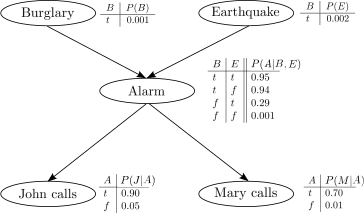
\includegraphics[width=7.5cm]{img/section3_fig5_v2_2}  
	%\end{center}
	

%\begin{equation}
	%\begin{array}{lll}
	%P(B|J=true, M=true) 
	%& = & \underbrace{ \alpha P(B, J=true, M=true) }_{
		%\substack{ \text{normalization} \\ \text{c.f. section 3.1.3}}} \\\\
	%& = & \underbrace{ \alpha \sum\limits_{a,e} P(B, e, a, 
				%J=true, M=true) }_{
		%\text{marginalization}} \\\\
	%& = & \alpha P(B) \sum\limits_e P(e) \sum\limits_a P(a|B,e) \\
	%&& \cdot P(J=true|a) P(M=true|a) \\\\
	%& = & \alpha \cdot \left \{ \begin{array}{ll}
			%0.00059224 & \text{for } B=true \\\\
			%0.0014919 & \text{for } B=false
		%\end{array} \right.
	%\end{array}
%\end{equation}
%\end{frame}

\begin{frame}\frametitle{\secname}
    
A factorization of the full joint distribution\footnote{See Ch. 14 from \citep{russell2016artificial} for more details.}:

\begin{equation}
P(X_{1},\ldots,X_{n}) = \prod_{i=1}^{n} P(X_{i} | parents(X_{i}))
\end{equation}
    
Remember: independence is important. Independence can be identified via the 
\underline{Markov blanket}

The Markov blanket of a node includes:
\begin{itemize}
\item its parents
\item its children
other parents of the children    
\end{itemize}
    
\end{frame}

\subsection{Preparations to perform inference}

\begin{frame}\frametitle{\subsecname}
    
    \begin{enumerate}
     \item use topological representation to ensure a compact representation.
     The purpose of topological sorting is to identify cliques in the chordal decomposable graph (next week)
     \item turn DAG into a \emph{moral graph} i.e. \\
     an undirected graph + new edges s.t. each node of the original DAG is now directly connected to the nodes of its \emph{Markov blanket}
     \item Perform inference efficiently (next week)\\
     \textcolor{gray}{ by applying \emph{message passing} on the \emph{Junction tree}}
    \end{enumerate}
    
\end{frame}

\subsubsection{Topological sorting}


% -----------------------------------------------------------------------------
\begin{frame} \frametitle{\subsubsecname}

\mode<presentation>{
	\begin{textblock}{}(10.5,10)
		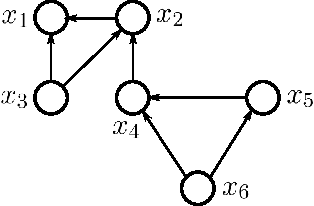
\includegraphics[width=4cm]{img/section3_fig17}
	\end{textblock}
	}

	\begin{itemize}
	\mode<presentation>{
		\item Factorization of the unconditional probability:
		$$
				P(X_1,\ldots, X_n) \quad=\quad 
				{\textstyle\prod\limits_{i=1}^n} P\big(X_i\,|\,parents(X_i)\big)
		$$
		\vspace{4mm}
		}
		
\mode<article>{
	\begin{figure}[h]
		 \centering
		 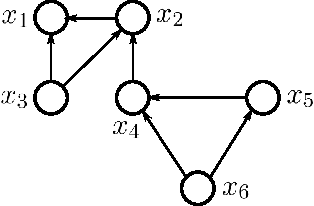
\includegraphics[width=0.4\textwidth]{img/section3_fig17}%
		 \caption{Example DAG}
	\end{figure}
}
		\item Edges should always be directed from nodes with lower 
			to nodes with higher indices.
		\vspace{8mm}
		\item Topological sorting: From parents to children:
			\begin{enumerate}
				\item select and queue a node without parents
				\item delete that node from the DAG
				\item repeat until DAG is empty
				\item renumber nodes
			\end{enumerate}
	\end{itemize}
\end{frame}


% -----------------------------------------------------------------------------
\begin{frame} \frametitle{\subsubsecname}
	\begin{minipage}{12.1cm}
		\begin{minipage}{7cm}
			\begin{itemize}
				\item example:
					\begin{itemize}
						\item ${\color{red}x_3},
							\visible<2->{x_6,}
							\visible<3->{x_5,}
							\visible<4->{x_4,}
							\visible<5->{x_2,}
							\visible<6->{x_1}$
					\end{itemize}
				\vspace{5mm}
				\item<7-> other possible topological orderings:
					\begin{itemize}
						\item $x_6,
							\visible<2->{x_5,}
							\visible<3->{x_4,}
							\visible<4->{{\color{red}x_3},}
							\visible<5->{x_2,}
							\visible<6->{x_1}$
						\item $x_6,
							\visible<2->{x_5,}
							\visible<3->{{\color{red}x_3},}
							\visible<4->{x_4,}
							\visible<5->{x_2,}
							\visible<6->{x_1}$
						\item $x_6,
							\visible<2->{{\color{red}x_3},}
							\visible<3->{x_5,}
							\visible<4->{x_4,}
							\visible<5->{x_2,}
							\visible<6->{x_1}$
					\end{itemize}
			\end{itemize}
		\end{minipage}
		\begin{minipage}{4cm}
			\includegraphics<1>[width=4cm]{img/section3_fig17_step1}
			\includegraphics<2>[width=4cm]{img/section3_fig17_step2}
			\includegraphics<3>[width=4cm]{img/section3_fig17_step3}
			\includegraphics<4>[width=4cm]{img/section3_fig17_step4}
			\includegraphics<5>[width=4cm]{img/section3_fig17_step5}
			\includegraphics<6>[width=4cm]{img/section3_fig17_step6}
			\mode<presentation>{
			\includegraphics<7>[width=4cm]{img/section3_fig17}
			}
		\end{minipage}
	\end{minipage}
\end{frame}

\begin{frame}

Exercise: topological sorting

\begin{figure}[h]
	\centering
	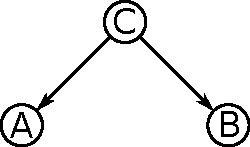
\includegraphics[width=0.3\linewidth]{img/cond}%
	\notesonly{
	\caption{
	DAG
	}%
	}%
    \label{fig:cond}%
\end{figure}

	\begin{itemize}
		\item Topological sorting: From parents to children:
			\begin{enumerate}
				\item select and queue a node without parents
				\item delete that node from the DAG
				\item repeat until DAG is empty
				\item renumber nodes
			\end{enumerate}
	\end{itemize}


\textbf{(see blackboard)}


\end{frame}


\begin{frame}

Exercise: topological sorting

\begin{figure}[h]
	\centering
	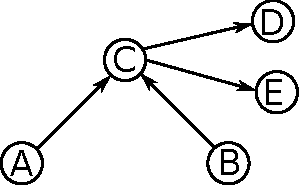
\includegraphics[width=0.3\linewidth]{img/dag1}%
	\notesonly{
	\caption{
	DAG
	}%
	}%
    \label{fig:cond}%
\end{figure}
\mode<presentation>{
	\begin{itemize}
		\item Topological sorting: From parents to children:
			\begin{enumerate}
				\item select and queue a node without parents
				\item delete that node from the DAG
				\item repeat until DAG is empty
				\item renumber nodes
			\end{enumerate}
	\end{itemize}
}

\textbf{(see blackboard)}


\end{frame}

\begin{frame}

Exercise: DAG (same as before) to moral graph

\mode<presentation>{
\begin{figure}[h]
	\centering
	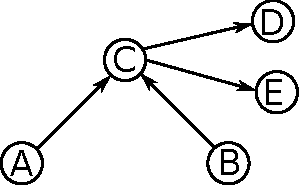
\includegraphics[width=0.3\linewidth]{img/dag1}%
	\notesonly{
	\caption{
	DAG
	}%
	}%
    \label{fig:cond}%
\end{figure}
}
\mode<presentation>{
\begin{enumerate}
\item make the edges undirected
\item identify the Markov blanket of each node (parents, children, other parents of the children)
\item add edges such that all nodes are directly connected to the Markov blanket.
\end{enumerate}
}

\textbf{(see blackboard)}
    
\end{frame}

\mode*

%\clearpage

\section{References}
\begin{frame}[allowframebreaks] \frametitle{References}
	\scriptsize
	\bibliographystyle{plainnat}
	\bibliography{bibliography}
\end{frame}

\end{rightcolumn}
\end{paracol}

\end{document}
